\chapter{Small worlds and affiliation networks}
\label{sw-affnets}

In order to assert that an actual network is a small-world network we should compare it against a null model. This null model is a random network with the same number of nodes and edges, but the edges assigned uniformly at random between the nodes. A small world network should be more highly clustered than its random counterpart and it should have similar short average path length. Building in this definition of smallwordiness, we can define the small world index ($Q$) as the division of the $CC_{ratio}$ by the $L_{ratio}$ \citep{watts:1999b,davis:2003,uzzi:2005,uzzi:2007}. If $Q > 1$ we can assert that the actual network under analysis is a small world network.

\begin{equation}
% \begin{split}
Q = \frac{CC_{ratio}}{L_{ratio}}
% \end{split}
\end{equation}

Where:

\begin{align}
CC_{ratio}& = \frac{CC_{actual}}{CC_{random}} &
L_{ratio}& = \frac{L_{actual}}{L_{random}} \nonumber \\
\end{align}

Affiliation networks contain two types of nodes: $N$ actors each of which belongs to one or more groups $M$. Such networks are bipartite or 2-mode because they contain two types of nodes and there are no edges between nodes of same type. We can obtain an unipartite or 1-mode network ---with only one type of nodes--- projecting the bipartite network on the actors' side or on the groups' side. This projection assumes that the actors are connected if they belong to the same group and that groups are connected if they share some actor, respectively.

Their statistical properties differ from unipartite networks. As \citet[83]{uzzi:2007} point out, affiliation networks, on the one hand, have higher clustering than unipartite networks because each actor's membership in a team makes them a fully connected clique in the one-mode projection, therefore an important part of the clustering is not due to ``the friends of an actor are friends themselves'' but to team topography. On the other hand, affiliation networks tend to have shorter average path lengths as the number of overlapping members between teams increase.

Although a common practice, it is well documented in the literature that there is an important lost of information when we perform a 1-mode projection from a 2-mode network \citep[324-325]{wasserman:1994}. Our approach to analyze the structure of the production process of the FOSS projects is to focus on the topology and the connectivity of 2-mode networks. \citet{robins:2004} redefined clustering coefficient in order to analyze 2-mode networks of directors and firms. Their approach is based in the analysis of network configurations or motifs.

\begin{figure}[h]
\begin{center}
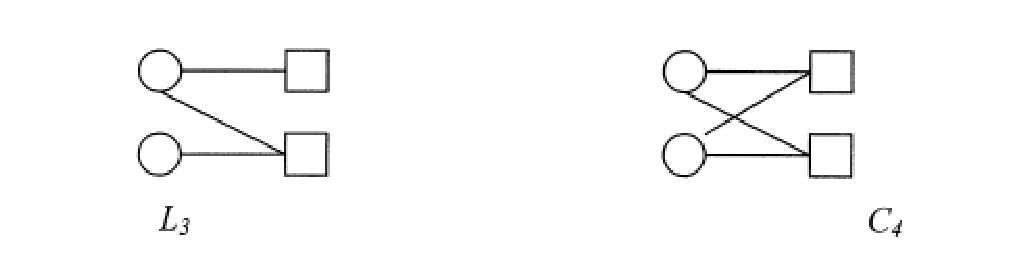
\includegraphics[scale=0.60]{figures/motifs}
\caption[Network motifs for bipartite networks.]{Relevant motifs in two mode network in order to calculate $CC_4$ \citep[78]{robins:2004}}
\label{fig:motifs}
\end{center}
\end{figure}

Figure \ref{fig:motifs} depicts the two relevant motifs or configurations in order to compute the bipartite clustering coefficient ($CC_4$). Three-paths ($L_3$) are composed by four nodes ---two of each type in the 2-mode network--- linked by three edges. \citeauthor{robins:2004} argue that the number of $L_3$ in 2-mode network is information lost in the 1-mode projection, they stress their importance: ``three-paths are important to connectivity, potentially providing short geodesics between directors and companies of which they are \emph{not} members. Long paths across the network of course must comprise several of these short three-paths, so we argue that the three-paths are precursors of global connectivity'' \citep[77-78]{robins:2004}.

Squares ($C_4$) are composed by four nodes ---two of each type--- linked by four edges. Squares are the simplest form of cycle in 2-mode networks and provide redundancy: when we perform the 1-mode projection, those four edges are represented by only one edge between the two nodes of the same type\footnote{If the projection is weighted the value of the edge will be 2, acknowledging that the two nodes are linked to two groups in the 2-mode network.}. \citet[79]{robins:2004} propose compute the bipartite clustering coefficient as depicted in equation \ref{e:robins}. 

\begin{equation}
\label{e:robins}
CC_4 = \frac{4 \times C_4}{L_3}
\end{equation}

\citet[79]{robins:2004} argue that ``high bipartite clustering indicates localized closeness and redundancy, just as is the case with triangles in 1-mode networks. [..] If the bipartite clustering coefficient is high, then many $L_3$ patterns are redundant. They do not provide new paths of connectivity across the bipartite graph. So for two bipartite graphs of similar size, the graph with the higher bipartite clustering ratio will show lower levels of connectivity''.
